%% Преамбула TeX-файла

% 1. Стиль и язык
\documentclass[utf8x, 12pt]{G7-32} % Стиль (по умолчанию будет 14pt)

% Остальные стандартные настройки убраны в preamble.inc.tex.
\sloppy

% Настройки стиля ГОСТ 7-32
% Для начала определяем, хотим мы или нет, чтобы рисунки и таблицы нумеровались в пределах раздела, или нам нужна сквозная нумерация.
\EqInChapter % формулы будут нумероваться в пределах раздела
\TableInChapter % таблицы будут нумероваться в пределах раздела
\PicInChapter % рисунки будут нумероваться в пределах раздела
\usepackage{slashbox}

% Добавляем гипертекстовое оглавление в PDF
\usepackage[
bookmarks=true, colorlinks=true, unicode=true,
urlcolor=black,linkcolor=black, anchorcolor=black,
citecolor=black, menucolor=black, filecolor=black,
]{hyperref}

% Изменение начертания шрифта --- после чего выглядит таймсоподобно.
% apt-get install scalable-cyrfonts-tex

\IfFileExists{cyrtimes.sty}
    {
        \usepackage{cyrtimespatched}
    }
    {
        % А если Times нету, то будет CM...
    }

\usepackage{graphicx}   % Пакет для включения рисунков

% С такими оно полями оно работает по-умолчанию:
% \RequirePackage[left=20mm,right=10mm,top=20mm,bottom=20mm,headsep=0pt]{geometry}
% Если вас тошнит от поля в 10мм --- увеличивайте до 20-ти, ну и про переплёт не забывайте:
\geometry{right=20mm}
\geometry{left=30mm}


% Пакет Tikz
\usepackage{tikz}
\usetikzlibrary{arrows,positioning,shadows}

% Произвольная нумерация списков.
\usepackage{enumerate}

% ячейки в несколько строчек
\usepackage{multirow}

% itemize внутри tabular
\usepackage{paralist,array}

% Центрирование подписей к плавающим окружениям
\usepackage[justification=centering]{caption}

% объявляем новую команду для переноса строки внутри ячейки таблицы
\newcommand{\specialcell}[2][c]{%
	\begin{tabular}[#1]{@{}c@{}}#2\end{tabular}}



% Настройки листингов.
\ifPDFTeX
% Листинги

\usepackage{listings}
\usepackage{wrapfig}
% Значения по умолчанию
\lstset{
  basicstyle= \footnotesize,
  breakatwhitespace=true,% разрыв строк только на whitespacce
  breaklines=true,       % переносить длинные строки
%   captionpos=b,          % подписи снизу -- вроде не надо
  inputencoding=koi8-r,
  numbers=left,          % нумерация слева
  numberstyle=\footnotesize,
  showspaces=false,      % показывать пробелы подчеркиваниями -- идиотизм 70-х годов
  showstringspaces=false,
  showtabs=false,        % и табы тоже
  stepnumber=1,
  tabsize=4,              % кому нужны табы по 8 символов?
  frame=single,
  escapeinside={(*}{*)}, %выделение
  literate={а}{{\selectfont\char224}}1
  {б}{{\selectfont\char225}}1
  {в}{{\selectfont\char226}}1
  {г}{{\selectfont\char227}}1
  {д}{{\selectfont\char228}}1
  {е}{{\selectfont\char229}}1
  {ё}{{\"e}}1
  {ж}{{\selectfont\char230}}1
  {з}{{\selectfont\char231}}1
  {и}{{\selectfont\char232}}1
  {й}{{\selectfont\char233}}1
  {к}{{\selectfont\char234}}1
  {л}{{\selectfont\char235}}1
  {м}{{\selectfont\char236}}1
  {н}{{\selectfont\char237}}1
  {о}{{\selectfont\char238}}1
  {п}{{\selectfont\char239}}1
  {р}{{\selectfont\char240}}1
  {с}{{\selectfont\char241}}1
  {т}{{\selectfont\char242}}1
  {у}{{\selectfont\char243}}1
  {ф}{{\selectfont\char244}}1
  {х}{{\selectfont\char245}}1
  {ц}{{\selectfont\char246}}1
  {ч}{{\selectfont\char247}}1
  {ш}{{\selectfont\char248}}1
  {щ}{{\selectfont\char249}}1
  {ъ}{{\selectfont\char250}}1
  {ы}{{\selectfont\char251}}1
  {ь}{{\selectfont\char252}}1
  {э}{{\selectfont\char253}}1
  {ю}{{\selectfont\char254}}1
  {я}{{\selectfont\char255}}1
  {А}{{\selectfont\char192}}1
  {Б}{{\selectfont\char193}}1
  {В}{{\selectfont\char194}}1
  {Г}{{\selectfont\char195}}1
  {Д}{{\selectfont\char196}}1
  {Е}{{\selectfont\char197}}1
  {Ё}{{\"E}}1
  {Ж}{{\selectfont\char198}}1
  {З}{{\selectfont\char199}}1
  {И}{{\selectfont\char200}}1
  {Й}{{\selectfont\char201}}1
  {К}{{\selectfont\char202}}1
  {Л}{{\selectfont\char203}}1
  {М}{{\selectfont\char204}}1
  {Н}{{\selectfont\char205}}1
  {О}{{\selectfont\char206}}1
  {П}{{\selectfont\char207}}1
  {Р}{{\selectfont\char208}}1
  {С}{{\selectfont\char209}}1
  {Т}{{\selectfont\char210}}1
  {У}{{\selectfont\char211}}1
  {Ф}{{\selectfont\char212}}1
  {Х}{{\selectfont\char213}}1
  {Ц}{{\selectfont\char214}}1
  {Ч}{{\selectfont\char215}}1
  {Ш}{{\selectfont\char216}}1
  {Щ}{{\selectfont\char217}}1
  {Ъ}{{\selectfont\char218}}1
  {Ы}{{\selectfont\char219}}1
  {Ь}{{\selectfont\char220}}1
  {Э}{{\selectfont\char221}}1
  {Ю}{{\selectfont\char222}}1
  {Я}{{\selectfont\char223}}1
}

% Стиль для псевдокода: строчки обычно короткие, поэтому размер шрифта побольше
\lstdefinestyle{pseudocode}{
  basicstyle=\small,
  keywordstyle=\color{black}\bfseries\underbar,
  language=Pseudocode,
  numberstyle=\footnotesize,
  commentstyle=\footnotesize\it
}

% Стиль для обычного кода: маленький шрифт
\lstdefinestyle{realcode}{
  basicstyle=\scriptsize,
  numberstyle=\footnotesize
}

% Стиль для коротких кусков обычного кода: средний шрифт
\lstdefinestyle{simplecode}{
  basicstyle=\footnotesize,
  numberstyle=\footnotesize
}

% Стиль для BNF
\lstdefinestyle{grammar}{
  basicstyle=\footnotesize,
  numberstyle=\footnotesize,
  stringstyle=\bfseries\ttfamily,
  language=BNF
}

% Определим свой язык для написания псевдокодов на основе Python
\lstdefinelanguage[]{Pseudocode}[]{Python}{
  morekeywords={each,empty,wait,do},% ключевые слова добавлять сюда
  morecomment=[s]{\{}{\}},% комменты {а-ля Pascal} смотрятся нагляднее
  literate=% а сюда добавлять операторы, которые хотите отображать как мат. символы
    {->}{\ensuremath{$\rightarrow$}~}2%
    {<-}{\ensuremath{$\leftarrow$}~}2%
    {:=}{\ensuremath{$\leftarrow$}~}2%
    {<--}{\ensuremath{$\Longleftarrow$}~}2%
}[keywords,comments]

% Свой язык для задания грамматик в BNF
\lstdefinelanguage[]{BNF}[]{}{
  morekeywords={},
  morecomment=[s]{@}{@},
  morestring=[b]",%
  literate=%
    {->}{\ensuremath{$\rightarrow$}~}2%
    {*}{\ensuremath{$^*$}~}2%
    {+}{\ensuremath{$^+$}~}2%
    {|}{\ensuremath{$|$}~}2%
}[keywords,comments,strings]

% Подписи к листингам на русском языке.
\renewcommand\lstlistingname{\cyr\CYRL\cyri\cyrs\cyrt\cyri\cyrn\cyrg}
\renewcommand\lstlistlistingname{\cyr\CYRL\cyri\cyrs\cyrt\cyri\cyrn\cyrg\cyri}

\else
\usepackage{local-minted}
\fi

% Полезные макросы листингов.
% Любимые команды
\newcommand{\Code}[1]{\textbf{#1}}


\begin{document}

\frontmatter 

% НАЧАЛО ТИТУЛЬНОГО ЛИСТА
% \noindent \begin{minipage}{0.15\textwidth}
% 	
\includegraphics[width=\linewidth]{img/b_logo}
% \end{minipage}
% \noindent\begin{minipage}{0.9\textwidth}\centering
% 	\textbf{Министерство науки и высшего образования Российской Федерации}\\
% 	\textbf{Федеральное государственное бюджетное образовательное учреждение высшего образования}\\
% 	\textbf{«Московский государственный технический университет имени Н.Э.~Баумана}\\
% 	\textbf{(национальный исследовательский университет)»}\\
% 	\textbf{(МГТУ им. Н.Э.~Баумана)}
% \end{minipage}

% \noindent\rule{18cm}{3pt}
% \newline
% \noindent ФАКУЛЬТЕТ $\underline{\text{«Информатика и системы управления»}}$ \newline
% \noindent КАФЕДРА $\underline{\text{«Программное обеспечение ЭВМ и информационные технологии»}}$\newline


% \begin{center}
% 	\noindent\begin{minipage}{1.2\textwidth}\centering
% 		\textbf{ОТЧЕТ ПО ЛАБОРАТОРНОЙ №2}\newline
% 		\textbf{По курсу: "Анализ алгоритмов"}\newline\newline\newline
% 	\end{minipage}
% \end{center}




% \noindent ~~Студент $\underline{\text{~~~~~~~~~~~~~~~~~~~~~~~~~~~~~~Сукочева Алис~~~~~~~~~~~~~~~~~~~~~~~~~~~~~~~~~~~~~~~~~~~~~~~~~~}}$

% \noindent ~~Группа $\underline{\text{~~~~~~~~~~~~~~~~~~~~~~~~~~~~~~~~~~~~~~ИУ7-53Б~~~~~~~~~~~~~~~~~~~~~~~~~~~~~~~~~~~~~~~~~~~~~~~~~~~~}}$

% \noindent ~~Название предприятия $\underline{\text{~~~~~~~~МГТУ им. Н. Э. Баумана, каф. ИУ7~~~~~~~~~~~~~~~~~~~~~~}}$

% \noindent ~~Тема $\underline{\text{~~~~~~~~~~~~~~~~~~~~~~~~~~~~~~~~Умножение матриц~~~~~~~~~~~~~~~~~~~~~~~~~~~~~~~~~~~~~~~}}$\newline


% \noindent\begin{tabular}{lcc}
% 	Студент: ~~~~~~~~~~~~~~~~~~~~~~~~~~~~~~~~~~~~~~~~~~~~~~~~~~~~~~~~ & $\underline{\text{~~~~~~~~~~~~~~~~}}$ & $\underline{\text{~~Сукочева А.~~}}$       \\
% 	                                                                  & \footnotesize подпись, дата           & \footnotesize Фамилия, И.О.                \\
% 	%& &  \\
% 	Преподаватель:                                                    & $\underline{\text{~~~~~~~~~~~~~~~~}}$ & $\underline{\text{~~~~Волкова Л.Л.~~~}}$   \\
% 	                                                                  & \footnotesize подпись, дата           & \footnotesize Фамилия, И. О.               \\
% 	Преподаватель:                                                    & $\underline{\text{~~~~~~~~~~~~~~~~}}$ & $\underline{\text{~~~~Строганов Ю.В.~~~}}$ \\
% 	                                                                  & \footnotesize подпись, дата           & \footnotesize Фамилия, И. О.               \\
% \end{tabular}


% \begin{center}
% 	\vfill
% 	Москва~---~\the\year
% 	~г.
% \end{center}

% \thispagestyle{empty}
% КОНЕЦ ТИТУЛЬНОГО ЛИСТА
1.

\tableofcontents

\Introduction

В настоящее время большую актуальность 
приобретает исследования выделения памяти многопоточным приложениям.
При этом отдельно рассматривают проблемы выделения 
виртуальной и физической памяти при выполнении процесса.

% особенности выделения вирт памяти на физич ? мы это не рассматривали 

% Сколько физич страниц в итоге выделяется процессе (это можно посмотреть ) - гипотетич

% Адресное пространство процесса состоит из виртуальной памяти, адресуемой
% процессом, и диапазона адресов в этой виртуальной памяти, которые
% разрешено использовать процессу. Данная курсовая работа предоставит 
% информацию, которая не доступна в режиме пользователя.

Целью данной работы является разработка загружаемого модуля ядра,
который будет предоставлять возможность пользователю мониторинга
виртуальной памяти и анализа количества выделенных страниц.

В данной работе также приведено исследование выделения виртуальной памяти процессам 
в зависимости от количества запрашиваемой памяти и от количества выполняемых потоков.

% В рамках выполнения работы необходимо решить следующие задачи.

% \begin{enumerate}
% 	\item 
% \end{enumerate}

\mainmatter % это включает нумерацию глав и секций в документе ниже


\chapter{Аналитический раздел}
\label{cha:analysis}

\section{ПОставновка задачи}

В соотв с заданием  на курс раб по курсу ос необходимо произвести исслед . выедления вирт памяти
многопоточным приложеям 

для решения щадачи необходмио 1 2 3....

метода лаба про форк карта (оптимизация форк) если не найду написать на почту 

изучить структуры (описываюшие едро) 
исследовать и тд

% \section{Адресное пространство процесса}

% Ядро управляет памятью пользовательских программ.
% Эта память называется адресным пространством процесса (process address space) 
% и выделяется операционной системой каждому пользовательскому процессу.
% Операционная система Linux является системой с поддержкой виртуальной памяти,
% т.е. в ней выполняется виртуализация ресурсов памяти среди всех процессов в системе.
% Для каждого процесса создается иллюзия того, что он один использует всю физическую память в системе.
% Адресное пространство одного процесса может значительно превышать объем физической памяти компьютера.

\subsection{Виртуальная адресное пространство}

Стали делить память на страницы. Можно выполнить программу, которая находится не целиком в памяти. 
Для этого нужно содержать части кода с которыми в текущий момент работает процессор.
Это воплотилось в понятие виртуальная память.

\textit{Виртуальная память} – память, размер которой превышает размер реального физического пространства.
Виртуальная память сама по себе ничего не хранит. 
Виртуальное адресное пространство — это абстракция, но оно определенным образом поставлено в соответствие физической памяти.

Загрузка частей программы в память выполняется по запросу. 
Т.е. соответствие части кода загружаемого по запросу, когда процессор обращается к этим частям кода.

\subsection{Таблица страниц}

Адресное пространство процесса и адресное пространство физической памяти делится на блоки равного размера. Блоки, на которые делится адресное пространство процесса называют страницами, а блоки на которые делится физическая память – кадрами, фреймами или блоками.

Виртуальный адрес состоит из двух частей:

\begin{itemize}
	\item p - номер страницы,
	\item d - смещение страницы.
\end{itemize}

На рис. \ref{fig:1} продемонстрировано отображение виртуальной памяти на физическую с помощью таблицы страниц.

\begin{figure}[ht!]
	\centering{
		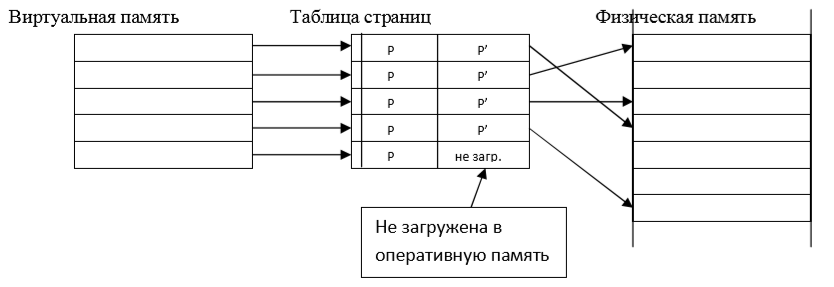
\includegraphics[width=0.8\textwidth]{img/1.png}
		\caption{Отображение виртуальной памяти на физическую с помощью таблицы страниц}
		\label{fig:1}}
\end{figure}

\newpage

% \subsection{Поле pgd}

С помощью таблиц страниц процессор осуществляет 
преобразование виртуального адреса в физический. 
У каждого процесса есть свой набор таблиц страниц.
Как только происходит переключение процесса (context switch), меняются и таблицы страниц. 
В Linux, указатель на таблицы страниц процесса хранится в поле pgd дескриптора памяти процесса. 
Каждой виртуальной странице соответствует одна запись в таблице страниц.

На рис. \ref{fig:2} показана 4-байтовая запись pgd.

\begin{figure}[ht!]
	\centering{
		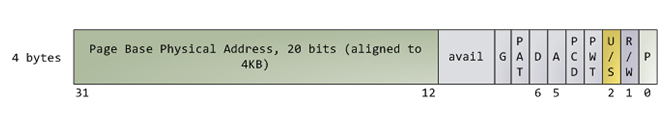
\includegraphics[width=1\textwidth]{img/2.jpg}
		\caption{4-байтовая запись pgd}
		\label{fig:2}}
\end{figure}

Флаг «P» говорит о том, находится ли страница в оперативной памяти или нет.
Когда данный флаг установлен в 0, доступ к соответствующей странице вызовет page fault.
Флаг «R/W» означает «запись/чтение»; если флаг не установлен, то к странице возможен доступ только на чтение.
Флаг «U/S» означает «пользователь/супервайзер»; если флаг не установлен, только код выполняющийся 
с уровнем привилегий 0 (т.е. ядро) может обратиться к данной странице.
Таким образом, данные флаги используются для того, чтобы реализовать концепцию адресного 
пространства доступного только на запись и пространства, которое доступно только для ядра.
Флаги «D» и «A» означают «dirty» и «accessed». «Dirty-страница» – эта та, в которую была недавно проведена запись, 
а «accessed»-страница – это страница, к которой было осуществлено обращение (чтение или запись). 
pgd хранит начальный физический адрес страницы в памяти.

При выполнении программы, которая находится не целиком в памяти, процесс потребует страницу, 
которой нет в оперативной памяти - возникнет исключение (страничная неудача - исправимое исключение), 
которое будет обработано в режиме ядра. В результате менеджер памяти попытается загрузить страницу 
в свободную память, а процесс на это время будет заблокирован. По завершении работы менеджера памяти страница
будет загружена и процесс будет продолжать выполнятся с той команды, на которой возникло исключение. 
Если свободная страница в физической памяти отсутствует, то менеджер памяти должен выбрать страницу для замещения.

Процесс может обращаться только к разрешенным областям памяти. 
Каждой области памяти назначаются определенные права доступа, такие как чтение, запись 
или выполнение, которые процесс должен неукоснительно соблюдать. 
Если процесс обращается по адресу, который не относится к разрешенной области памяти, 
или если доступ к разрешенной области памяти выполняется некорректным образом, ядро уничтожает такой
процесс с сообщением «Segmentation Fault» (Ошибка сегментации).

В областях памяти может содержаться вся нужная процессу информация, такая как:

\begin{itemize}
	\item машинный код, загруженный из исполняемого файла в область памяти процесса, которая называется сегментом кода (text section);
	\item инициализированные переменные, загруженные из исполняемого файла в область памяти процесса, которая называется сегментом данных (data section);
	\item страницы памяти, заполненные нулями, в которых содержатся неинициализированные глобальные переменные программы. Эта область памяти называется сегментом bss 1 (bss section);
	\item страницы памяти, заполненные нулями, в которых находится пользовательский стек процесса;
	\item дополнительные сегменты кода, данных и BSS для каждой совместно используемой библиотеки, такой как библиотека libc и динамический компоновщик, которые загружаются в адресное пространство процесса.
\end{itemize}

\section{Структуры ядра}

\subsection{Структура task\_struct}

Список процессов хранится в ядре в виде циклического двухсвязного списка, 
который называется списком задач (task list). 
Каждый элемент этого списка описывает один
запущенный процесс и называется дескриптором процесса. Дескриптор процесса имеет
тип task\_struct, структура которого описана в файле <linux/sched.h>. 
Дескриптор процесса содержит всю информацию об определенном процессе.
В дескрипторе процесса содержатся данные, которые описывают выполняющуюся
программу, — открытые файлы, адресное пространство процесса, сигналы, ожидающие
обработки, состояние процесса и многое другое (рис. \ref{fig:3}). 
На листинге 1.1 представлена часть структуры task\_struct.

\begin{figure}[ht!]
	\centering{
		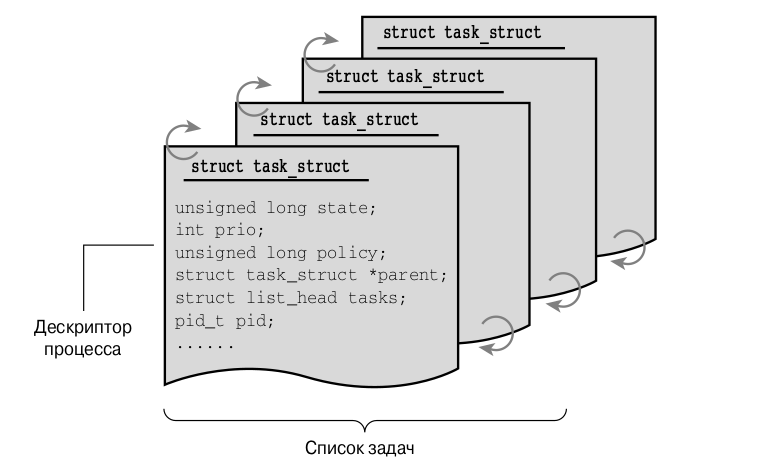
\includegraphics[width=1\textwidth]{img/3.png}
		\caption{Дескриптор процесса и список задач}
		\label{fig:3}}
\end{figure}

\newpage

\begin{lstlisting}[language=c, label=some-code, caption=Структура task\_struct]
struct task_struct {	
	void				*stack;
	refcount_t			usage;
	unsigned int			flags;
	unsigned int			ptrace;
	struct task_struct		*last_wakee;

	...

	unsigned int			policy;

	struct list_head		tasks;

	struct mm_struct		*mm;
	struct mm_struct		*active_mm;

	/* Per-thread vma caching: */
	struct vmacache			vmacache;

	int				exit_state;
	int				exit_code;
	int				exit_signal;

	pid_t				pid;
	pid_t				tgid;


	/* Real parent process: */
	struct task_struct __rcu	*real_parent;

	/* Recipient of SIGCHLD, wait4() reports: */
	struct task_struct __rcu	*parent;

	/*
	* Children/sibling form the list of natural children:
	*/
	struct list_head		children;
	struct list_head		sibling;
	struct task_struct		*group_leader;

	/* Filesystem information: */
	struct fs_struct		*fs;

	/* Open file information: */
	struct files_struct		*files;

	/* Namespaces: */
	struct nsproxy			*nsproxy;

	/* Signal handlers: */
	struct signal_struct		*signal;
	struct sighand_struct		*sighand;
	sigset_t			blocked;
	sigset_t			real_blocked;

	/* VM state: */
	struct reclaim_state		*reclaim_state;

	struct backing_dev_info		*backing_dev_info;

	struct io_context		*io_context;
	
	...	

};
\end{lstlisting}

\subsection{Структура mm\_struct.}

Адресное пространство процесса представляется в ядре в виде структуры данных, 
которая называется дескриптором памяти (memory descriptor). 
В этой структуре содержится вся информация, относящаяся к адресному пространству процесса. 
Дескриптор памяти представляется с помощью структуры mm\_struct,
которая определена в файле <linux/mm\_types.h>. 
Указатель на данную структуру содерержится в поле mm структуры task\_struct.  
Структура вместе с поясняющими комментариями по каждому полю приведена на листинге 1.2

\begin{lstlisting}[language=c, label=some-code, caption=Структура mm\_struct]
struct mm_struct {
	struct vm_area_struct *mmap; 
	/* Список областей памяти */
	struct rb_root mm_rb; 
	/* Красно-черное дерево областей памяти */
	struct vm_area_struct *mmap_cache;
	/* Последняя использованная область памяти */
	unsigned long free_area_cache; 
	/* Первый незанятый участок адресного пространства */
	pgd_t *pgd;
	/* Глобальный каталог страниц */
	atomic_t mm_users; 
	/* Счетчик использования адресного пространства */
	atomic_t mm_count; 
	/* Основной счетчик использования */
	int map_count; 
	/* Количество областей памяти */
	struct rw_semaphore mmap_sem; 
	/* Семафор для областей памяти */
	spinlock_t page_table_lock; 
	/* Спин-блокировка таблиц страниц */
	struct list_head mmlist;
	/* Список всех структур mm_struct */
	unsigned long start_code;
	/* Начальный адрес сегмента кода */
	unsigned long end_code;
	/* Конечный адрес сегмента кода */
	unsigned long start_data;
	/* Начальный адрес сегмента данных */
	unsigned long end_data;
	/* Конечный адрес сегмента данных */
	unsigned long start_brk;
	/* Начальный адрес сегмента "кучи" */
	unsigned long brk;
	/* Конечный адрес сегмента "кучи" */
	unsigned long start_stack;
	/* Начало стека процесса */
	unsigned long arg_start; 
	/* Начальный адрес области аргументов */
	unsigned long arg_end;
	/* Конечный адрес области аргументов */
	unsigned long env_start; 
	/* Начальный адрес области переменных среды */
	unsigned long env_end;
	/* Конечный адрес области переменных среды */
	unsigned long rss;
	/* Количество распределенных физических страниц памяти */
	unsigned long total_vm; 
	/* Общее количество страниц памяти */
	unsigned long locked_vm; 
	/* Количество заблокированных страниц памяти */
	unsigned long saved_auxv[AT_VECTOR_SIZE]; 
	/* Сохраненный вектор auxv */
	cpumask_t cpu_vm_mask;
	/* Маска отложенного переключения буфера TLB */
	mm_context_t context; 
	/* Данные, специфичные для аппаратной платформы */
	unsigned long  flags;
	/* Флаги состояния */
	int core_waiters;
	/* количество потоков, ожидающих создания файла дампа */
	struct core_state *core_state; 
	/* Поддержка дампа */
	spinlock_t ioctx_lock; 
	/* Блокировка списка асинхронного ввода-вывода (AIO) */
	struct hlist_head ioctx_list; 
	/* Список асинхронного ввода-вывода (AIO) */
};
\end{lstlisting}

В поле mm\_users хранится количество процессов, в которых используется данное
адресное пространство. Например, если одно и то же адресное пространство 
используется в двух потоках, значение поля mm\_users равно 2.

В полях mmap и mm\_rb хранятся ссылки на две различные структуры данных, 
содержащие одну и ту же информацию: информацию обо всех областях памяти в 
соответствующем адресном пространстве. В первой структуре эта информация 
хранится в виде связанного списка, а во второй — в виде красно-черного дерева. 
Поскольку красно-черное дерево — это разновидность двоичного дерева, 
то, как и для всех типов двоичных деревьев,
количество операций поиска заданного элемента в нем подчиняется закону O(log(n)).

Все структуры mm\_struct объединены в двухсвязный список с помощью полей mmlist.

\subsection{Структура vm\_area\_struct}

Области памяти (memory areas) представляются с помощью структуры 
vm\_area\_struct, которая определена в файле <linux/mm\_types.h>.

Структура vm\_area\_struct используется для описания одной непрерывной 
области памяти в данном адресном пространстве. В ядре каждая область памяти считается
уникальным объектом. Для каждой области памяти определены некоторые общие 
свойства, такие как права доступа и набор соответствующих операций. Таким образом, 
каждая структура VMA может представлять различный тип области памяти, например 
файлы, отображаемые в память, или стек пользовательского приложения.
Структура vm\_area\_struct приведена на листинге 1.3.

\begin{lstlisting}[language=c, label=some-code, caption=Структура vm\_area\_struct]
struct vm_area_struct {
	struct mm_struct *vm_mm;
	/* Соответствующая структура mm_struct */
	unsigned long vm_start;/* Начало диапазона адресов (включительно) */
	unsigned long vm_end; /* Конец диапазона адресов (исключая) */
	struct vm_area_struct *vm_next; /* Список областей VMA */
	pgprot_t vm_page_prot; /* Права доступа */
	unsigned long vm_flags;/* Флаги */
	struct rb_node vm_rb; /* Узел текущей области VMA в дереве */
	union {
		/* Связь с address_space->i_mmap или i_mmap_nonlinear */
		struct {
			struct list_head list;
			void *parent;
			struct vm_area_struct *head;
		} vm_set;

		struct prio_tree_node prio_tree_node;
	} shared;
	struct list_head anon_vma_node; /* Элемент анонимной области */
	struct anon_vma *anon_vma; /* Объект анонимной VMA */
	struct vm_operations_struct *vm_ops; /* Связанные операции */
	unsigned long vm_pgoff; /* Смещение в файле */
	struct file *vm_file; /* Отображенный файл (если есть) */
	void *vm_private_data; /* Частные данные */
};
\end{lstlisting}

\subsection{Взаимосвязь приведенных структур}

Взаимосвязь приведенных структур продемонстрирована на рис. \ref{fig:4}

\begin{figure}[ht!]
	\centering{
		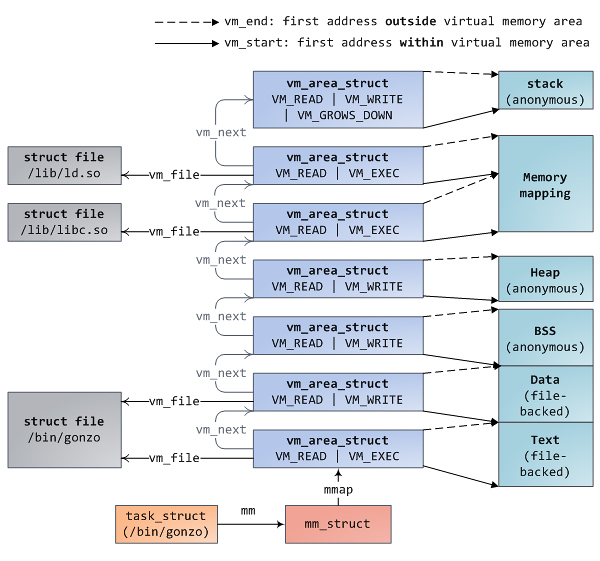
\includegraphics[width=0.7\textwidth]{img/4.jpg}
		\caption{Взаимосвязь приведенных структур}
		\label{fig:4}}
\end{figure}

\newpage

\section{Прерывания}

Прерывания делятся на:

\begin{itemize}
	\item исключения (деление на ноль, переполнение стека), синхронные;
	\item системные вызовы (программные) - вызываются с помощью соответствующей команды из программы (int 21h), синхронные;
	\item аппаратные прерывания (прерывания от системного таймера, клавиатуры), асинхронные. 
\end{itemize}

Прерывания делятся на 2 группы:

\begin{itemize}
	\item быстрые;
	\item медленные. 
\end{itemize}

Для того чтобы сократить время обработки медленных прерываний, они делятся на 2 части:

\begin{itemize}
	\item top half, верхняя половина, запускается в результате получения процессором сигнала прерывания;
	\item bottom half, нижняя половина, отложенные вызовы.
\end{itemize}

Существует несколько способов реализации “нижней половины“
обработчика: 
\begin{itemize}
	\item softirq;
	\item тасклет (tasklet);
	\item очереди работ (workqueue).
\end{itemize}

\subsection{Обработчики аппаратных прерываний}

Обработчик прерывания должен выполнять минимальный объем действий и завершаться как можно быстрее.
Обычно такой обработчик прерывания сохраняет данные, поступившие от внешнего устройства, в буфере ядра. 
Но для того чтобы обработать прерывания полностью, обработчик аппаратного прерывания должен 
инициализировать постановку в очередь на выполнение отложенное действие.

\subsection{Очереди работ}

Очереди работ являются обобщенным механизмом отложенного выполнения, в котором 
функция обработчика, реализующая соответствующие действия, может блокироваться.

struct workqueue\_struct - описывает очередь работ.

\begin{lstlisting}[language=c, label=some-code, caption=Структура workqueue\_struct]
struct workqueue_struct {
	struct list_head    pwqs;        /* WR: all pwqs of this wq */
	struct list_head    list;        /* PR: list of all workqueues */
	...
	struct pool_workqueue    *dfl_pwq;    /* PW: only for unbound wqs */
	...
	struct pool_workqueue __percpu *cpu_pwqs; /* I: per-cpu pwqs */
	...
	};
\end{lstlisting}

struct work\_struct - описывает работу (обработчик нижней половины).

\begin{lstlisting}[language=c, label=some-code, caption=Структура workqueue\_struct]
struct work_struct {
	atomic_long_t data;
	struct list_head entry;
	work_func_t func;
	...
};
\end{lstlisting}

Работа может инициализироваться 2-мя способами:

\begin{itemize}
	\item статически;
	\item динамически.
\end{itemize}

При статической инициализации используется макрос:

\begin{lstlisting}[language=c, label=some-code, caption=статическая инициализация]
	DECLARE_WORK(name, void (*func)(void *));
\end{lstlisting}

где: name – имя структуры work\_struct, func – функция, которая вызывается из workqueue – обработчик нижней половины.

При динамической инициализации используются макросы:

\begin{lstlisting}[language=c, label=some-code, caption=динамическая инициализация]
	INIT_WORK(sruct work_struct *work, void (*func)(void),void *data);
\end{lstlisting}

После того, как будет инициализирована структура для объекта work, следующим шагом будет помещение этой структуры в очередь работ. 
Это можно сделать несколькими способами. 
Во-первых, можно добавить работу (объект work) в очередь работ с помощью функции queue\_work (которая назначает работу текущему процессору). 
Во-вторых, можно с помощью функции queue\_work\_on указать процессор, на котором будет выполняться обработчик.

\section{Вывод}

Были рассмотрены основополагающие материалы, которые в дальнейшем потребуются при реализации 
загружаемого модуля ядра.




\chapter{ Констукторский раздел}
\label{cha:design}

\section{Требования к программе}

Необходимо реализовать загружаемый модуль ядра, который будет ... TODO:
TODO: блок схема для загружаемого модуля ядра

\section{Анализируемая программа}

В качестве анализируемой программы  была выбрана программа, 
которая запускала n потоков. 
Каждый поток создавал свой собственный кольцевой односвязный список.
Далее каждый поток пробегался по всему своему односвязному списку 
и обновлял значения (заполнял рандомными значениями).
После обновления списка в конец добавлялся новый узел 
и приведенные выше операции повторялись вновь. 
На рис. \ref{fig:5} показан кольцевой односвязный список, использующийся в анализируемой программе.

\begin{figure}[ht!]
	\centering{
		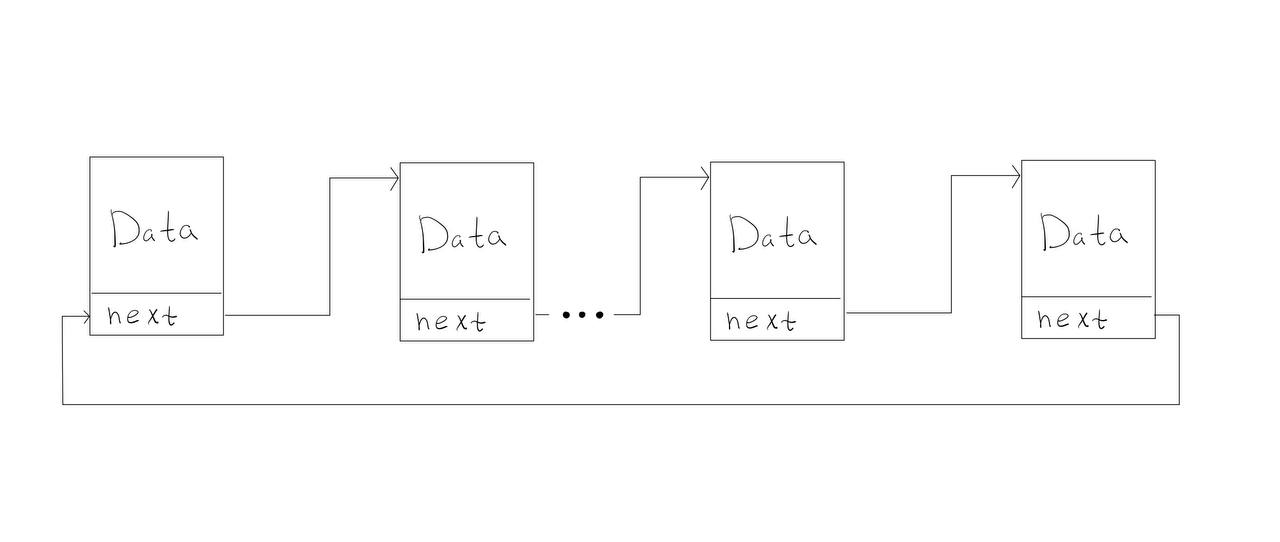
\includegraphics[width=1\textwidth]{img/5.jpeg}
		\caption{Кольцевой односвязный список}
		\label{fig:5}}
\end{figure}

На рис. \ref{fig:6} блок-схема алгоритма, который выполняет каждый поток. 

\begin{figure}[ht!]
	\centering{
		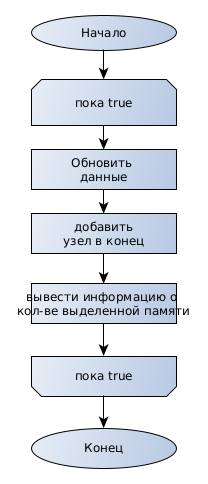
\includegraphics[width=0.4\textwidth]{img/6.png}
		\caption{Блок-схема алгоритма выполнения потока}
		\label{fig:6}}
\end{figure}



\section{Вывод}

В данном разделе было рассмотрено ...







\chapter{Технологический раздел}
\label{cha:design}

\section{Выбор языка программирования и среды разработки}

В данной курсовой работе использовался язык программирования - c \cite{bib1}.

В качестве среды разработки я использовала Visual Studio Code \cite{bib2}, т.к. считаю его достаточно удобным и легким.
Visual Studio Code подходит не только для  Windows \cite{bib3}, но и для Linux \cite{bib4}, это еще одна причина, по которой я выбрала VS code,
т.к. у меня установлена ОС Ubuntu 18.04.4 \cite{bib5}.

\section{Структура курсового проекта}

Курсовой проект состоит из:

\begin{itemize}
	\item md.c - загружаемого модуля ядра;
	\item my\_mem\_prog.c - анализируемой программы.
	\item additional\_program.с - дополнительной программы, позволяющей выделять 
	необходимое количество памяти, для дальнейшего анализа.
\end{itemize}

\section{Листинг загружаемого модуля ядра}

На листинге 3.1 приведен код загружаемого моду ядра. 

\begin{lstlisting}[language=c, label=some-code, caption=Загружаемый модуль ядра]
MODULE_LICENSE("GPL");
MODULE_AUTHOR("Alice");
MODULE_DESCRIPTION("Coursework BMSTU");

#define KBD_DATA_REG 0x60 /* I/O port for keyboard data */
#define KBD_SCANCODE_MASK 0x7f
#define KBD_STATUS_MASK 0x80


#define ANALYSIS_PROGRAM_NAME "my_mem_prog"

#define MONITORING_SCANCODE 1 // "[ESC]"

unsigned int my_irq = 1; // Прерывание от клавиатуры.

static struct workqueue_struct *my_wq; //очередь работ
struct task_struct *task = NULL;
char current_scancode;

bool find_user_task_struct(char* prog_name);
static void my_wq_function(struct work_struct *work);
irqreturn_t irq_handler(int irq, void *dev, struct pt_regs *regs);
void update_info_about_mem(struct mm_struct *info_about_mem);

DECLARE_WORK(my_work, my_wq_function);

unsigned long  total_vm_old;
unsigned long  locked_vm_old;
int  map_count_old;
unsigned long  all_brk_old;

void info_about_mm(void)
{
	struct mm_struct *info_about_mem; 
	bool is_new_data = false;

	unsigned long  total_vm_current;
	unsigned long  locked_vm_current;
	int map_count_current;
	unsigned long  all_brk_current;

	if (find_user_task_struct(ANALYSIS_PROGRAM_NAME) == false)
	{
		printk(KERN_INFO "+Module: find_user_task_struct is false");
		return;
	}

	info_about_mem = task->mm;

	total_vm_current = info_about_mem->total_vm;
	locked_vm_current = info_about_mem->locked_vm;
	map_count_current = info_about_mem->map_count;
	all_brk_current = info_about_mem->brk - info_about_mem->start_brk;
	
	// update_info_about_mem(info_about_mem);

	if (total_vm_old > total_vm_current)
	{
		total_vm_old = total_vm_current;
		return;
	}

	if (all_brk_old > all_brk_current)
	{
		all_brk_old = all_brk_current;
		return;
	}


	if (total_vm_current != total_vm_old)
	{
		printk(KERN_INFO "+Module: Общее количество страниц памяти: было: %lu; стало:%lu; разница:%lu", total_vm_old, total_vm_current, total_vm_current - total_vm_old);
		total_vm_old = total_vm_current;
		is_new_data = true;
	}

	if (all_brk_current != all_brk_old)
	{
		printk(KERN_INFO "+Module: Используется сегментом кучи: было: %lu; стало:%lu; разница:%lu", all_brk_old, all_brk_current, all_brk_current - all_brk_old);
		all_brk_old = all_brk_current;
		is_new_data = true;
	}

	if (!is_new_data)
	{
		printk(KERN_INFO "+Module: Нет изменений");
	}
}

static void my_wq_function(struct work_struct *work) // вызываемая функция
{
	int scan_normal;

	if (!(current_scancode & KBD_STATUS_MASK))
	{
		scan_normal = current_scancode & KBD_SCANCODE_MASK;

		if (scan_normal == MONITORING_SCANCODE)
		{
			info_about_mm();
		}
	}
}

irqreturn_t irq_handler(int irq, void *dev, struct pt_regs *regs)
{
	if (irq == my_irq)
	{		
		// Получаем скан-код нажатой клавиши.
		current_scancode = inb(KBD_DATA_REG);
		queue_work(my_wq, &my_work);

		return IRQ_HANDLED; // прерывание обработано
	}
	else
		return IRQ_NONE; // прерывание не обработано
}

bool find_user_task_struct(char* prog_name)
{
	struct task_struct *current_task = &init_task;

	do {
		if (!strcmp(current_task->comm, prog_name))
		{
			task = current_task;
			return true;
		}
	} while ((current_task = next_task(current_task)) != &init_task);

	return false;
}

void update_info_about_mem(struct mm_struct *info_about_mem)
{
	atomic_t mm_users; 
	int counter;

	mm_users = info_about_mem->mm_users; /* Счетчик использования адресного пространства */
	counter = mm_users.counter;

	total_vm_old = info_about_mem->total_vm;
	locked_vm_old = info_about_mem->locked_vm;
	map_count_old = info_about_mem->map_count;
	all_brk_old = info_about_mem->brk - info_about_mem->start_brk;

	printk(KERN_INFO "+Module: Количество процессов, в которых используется данное адресное пространство: %d", counter);

	printk(KERN_INFO "+Module: Общее количество страниц памяти = %lu ", total_vm_old);
	printk(KERN_INFO "+Module: Количество заблокированных страниц памяти = %lu ", locked_vm_old);
	printk(KERN_INFO "+Module: Количество областей памяти: %d", map_count_old);

	printk(KERN_INFO "+Module: Используется сегментом кучи: %lu", all_brk_old);
	printk(KERN_INFO "+Module: Используется сегментом кода: %lu", info_about_mem->end_code - info_about_mem->start_code);
	printk(KERN_INFO "+Module: Используется сегментом данных: %lu", info_about_mem->end_data - info_about_mem->start_data);
}


void first_proc(void)
{
	struct mm_struct *info_about_mem; 


	if (find_user_task_struct(ANALYSIS_PROGRAM_NAME) == false)
	{
		printk(KERN_INFO "+Module: find_user_task_struct is false");
		return;
	}

	info_about_mem = task->mm;

	update_info_about_mem(info_about_mem);
}

static int __init md_init(void)
{
	// регистрация обработчика прерывания
	if (request_irq(
			my_irq,						/* номер irq */
			(irq_handler_t)irq_handler, /* наш обработчик */
			IRQF_SHARED,				/* линия может быть раздедена, IRQ
										(разрешено совместное использование)*/
			"my_irq_handler",			/* имя устройства (можно потом посмотреть в /proc/interrupts)*/
			(void *)(irq_handler)))		/* Последний параметр (идентификатор устройства) irq_handler нужен
										для того, чтобы можно отключить с помощью free_irq  */
	{
		printk(" + Error request_irq");
		return -1;
	}

	my_wq = create_workqueue("my_queue"); //создание очереди работ
	if (my_wq)
	{
		printk(KERN_INFO "Module: workqueue created!\n");
	}
	else
	{
		free_irq(my_irq, irq_handler); // Отключение обработчика прерывания.
		printk(KERN_INFO "Module: error create_workqueue()!\n");
		return -1;
	}

	first_proc();
	// find_user_task_struct(ANALYSIS_PROGRAM_NAME);

	printk(KERN_INFO "Module: module loaded!\n");
	return 0;
}

static void __exit md_exit(void)
{
	// Принудительно завершаем все работы в очереди.
	// Вызывающий блок блокируется до тех пор, пока операция не будет завершена.
	flush_workqueue(my_wq);
	destroy_workqueue(my_wq);

	// my_irq - номер прерывания.
	// irq_handler - идентификатор устройства.
	free_irq(my_irq, irq_handler); // Отключение обработчика прерывания.
	
	printk(KERN_INFO "Module: unloaded!\n");
}

module_init(md_init);
module_exit(md_exit);
\end{lstlisting}

\section{Анализируемая программа}

На листинге 3.2 приведен код анализируемой программы. 
% gcc pthread_example.c -pthread -o my_mem_prog

\begin{lstlisting}[language=c, label=some-code, caption=Анализируемая программа]
#include <stdio.h>
#include <stdlib.h>
#include <time.h>
#include <unistd.h>
#include <errno.h>  
#include <pthread.h>

#define SUCCESS 0

#define ERROR_CREATE_THREAD -11
#define ERROR_JOIN_THREAD   -12

#define VALUE_SIZE 64
#define PTHREAD_COUNT 3
#define SLEEP_TIME 3

#define GET_RAND_NUMBER(min, max) (rand() % (max - min + 1) + min)

typedef struct Node {
	int *value; // VALUE_SIZE
	struct Node *next; // 8 byte
} Node;

Node *create()
{
	Node *node = (Node*)malloc(sizeof(Node));
	node->value = (int*)malloc(VALUE_SIZE * sizeof(int)); // VALUE_SIZE * 4 (при 64 == 256)
	node->next = NULL;
	return node;
}

void add_to_end(Node *node)
{
	Node *new_node = create();
	node->next = new_node;
}

void output_data(int *data)
{
	for (int i = 0; i < VALUE_SIZE; i++)
	{
		printf("%d ", data[i]);
	}
	printf("\n");
}

void output(Node *node)
{
	while(node != NULL)
	{
		output_data(node->value);
		node = node->next;
	}
	printf("\n\n");
}

void generate_random_values(Node *node)
{
	for (int i = 0; i < VALUE_SIZE; i++)
	{
		node->value[i] = GET_RAND_NUMBER(0, 100);
	}
}

void update_list(Node *node)
{
	while(node != NULL)
	{	
		generate_random_values(node);
		node = node->next;
	}
}

int msleep(long msec)
{
	struct timespec ts;
	int res;

	if (msec < 0)
	{
		errno = EINVAL;
		return -1;
	}

	ts.tv_sec = msec / 1000;
	ts.tv_nsec = (msec % 1000) * 1000000;

	do {
		res = nanosleep(&ts, &ts);
	} while (res && errno == EINTR);

	return res;
}

void process(char* name)
{
	Node *first = create();
	Node *current_node = first;

	long long int i = 0;
	while (1)
	{
		update_list(first);

		add_to_end(current_node);
		
		current_node = current_node->next;
		
		i++;
		if (!(i % 16))
		{
			printf("1 kilobytes\n");
		}

		long long int byte = (256 + 8) * i;
		printf(" %s byte = %lld kilobyte = %lld ",name, byte, byte / 1024);
		printf("pages = %lld \n", byte / 1024 / 4);
		msleep(SLEEP_TIME);
	}
}
	
void* do_pthread(void *args) 
{
	process((char*)args);
	return SUCCESS;
}

int main() 
{
	printf("Start program");
	srand(time(NULL));
	setbuf(stdout, NULL);
	
	pthread_t threads[PTHREAD_COUNT];
	char* names[5] = {"1", "2", "3", "4", "5"};

	int status;
	int status_addr;

	for (int i = 0; i < PTHREAD_COUNT; i++)
	{
		status = pthread_create(&threads[i], NULL, do_pthread, names[i]);
		if (status != 0) {
			printf("main error: can't create thread, status = %d\n", status);
			exit(ERROR_CREATE_THREAD);
		}
	}

	do_pthread("Main pthread"); 
}
\end{lstlisting}

\section{Вспомогательная программа}

На листинге 3.3 приведена вспомогательная программа.
Она предоставляет возможность выделения памяти, размер которой равен 1024 * 4 * n байт (n страниц). 
Где n - число, которое вводит пользователь.

\begin{lstlisting}[language=c, label=some-code, caption=Вспомогательная программа]
#include <stdio.h>
#include <stdlib.h>
#include <time.h>

#define PAGE_SIZE 4 * 1024 // 4 kilobyte
#define OK 0

void create(int page_count)
{
	void* mem = (void*)malloc(PAGE_SIZE * page_count);
	printf("malloc (%d pages)\n", page_count);
}

void process(void)
{
	int page_count = 1;
	while (page_count)
	{
		create(page_count);
		printf("Input page count (0 to exit) : ");
		scanf("%d", &page_count);
	}
}

int main()
{
	srand(time(NULL));
	setbuf(stdout, NULL);
	process();
	return OK;
}
\end{lstlisting}


% \section{Сведения о модулях программы}

% Данная программа разбита на модули:

% \begin{itemize}
% 	\item main.py - Файл, содержащий точку входа в программу. В нем происходит общение с пользователем и вызов алгоритмов;
% \end{itemize}

% На листингах 3.1-3.6 представлены 

% % \begin{lstlisting}[label=some-code,caption=Главная функция main]
% % \end{lstlisting}

% \section{Тестирование}

% В данном разделе будет приведена таблица 
% % \ref{table:ref1}, в которой четко отражено тестирование программы. ы

\section{Вывод}

В данном разделе был выбран язык программирования и среда разработки.
А также представлены листинги.
\chapter{Экспериментальная часть}

\section{Анализ увелечения количества страниц от количества потоков}

На рис. \ref{fig:analysis_pthread_count} демонстрируется
увеличение количества страниц от количества потоков (при первом запуске программы).

При одном главном потоке выделяется 1675 страниц.

При двух потоках выделяется 20108 страниц (примерно в 12 раз больше, чем при одном потоке).

Далее при увеличении количества потоков количество страниц увеличивается на 18433 страницы.

При единственном главном потоке (когда не создаются дочерние потоки) 
выделяется определенное количество страниц. 
Далее при первом вызове функции pthread\_create выделяется некоторое количество страниц.
Все последующие вызовы функции pthread\_create будут запрашивать 
определенное одинаковое количество страниц. 


\begin{figure}[ht!]
	\centering{
		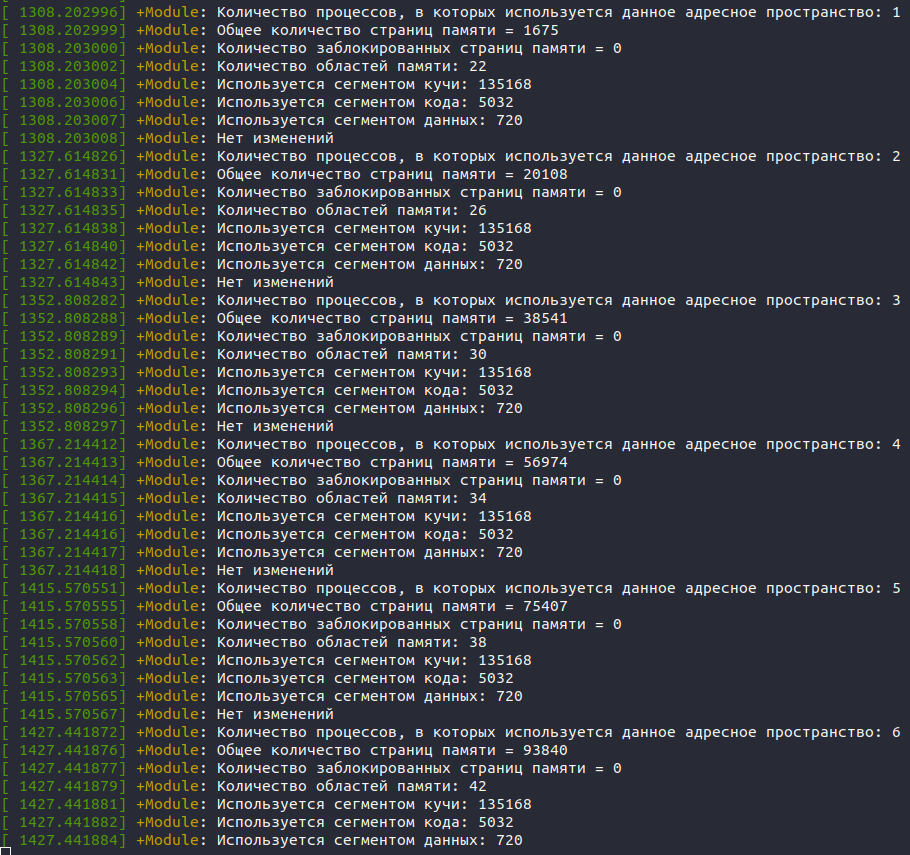
\includegraphics[width=0.95\textwidth]{img/analysis_pthread_count.png}
		\caption{Демонстрация увелечения количества страниц от количества потоков}
		\label{fig:analysis_pthread_count}}
\end{figure}

\newpage

// TODO: Указать размер  выделяемой памяти

\section{Анализ увелечения количества страниц программы, описанной выше}

На рис. \ref{fig:analysis_program} демонстрируется увеличение количества страниц 
при анализе описанной выше программы (при одном потоке).

Видно, что программе выделяется 33 страницы. 
Так же видно, что увеличивается размер кучи. 
Он увеличивается на 135168, что равно 33 * 4 * 1024, т.е. все 33 страницы выделяются под кучу.

\begin{figure}[ht!]
	\centering{
		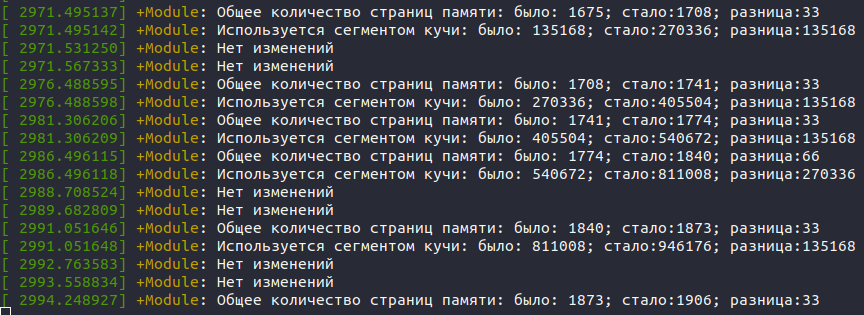
\includegraphics[width=1\textwidth]{img/analysis_program.png}
		\caption{Демонстрация увеличение количества страниц при анализе описанной выше программы}
		\label{fig:analysis_program}}
\end{figure}

\newpage

\section{Анализ увелечения количества страниц программы, описанной выше при увеличении количества потоков}

На рис. \ref{fig:analysis_program2} демонстрируется увеличение количества страниц 
при анализе описанной выше программы при увеличении количества потоков от 1 до 4.

Видно, что независимо, от изначального количества потоков программе выделяется 33 страницы. 

\begin{figure}[ht!]
	\centering{
		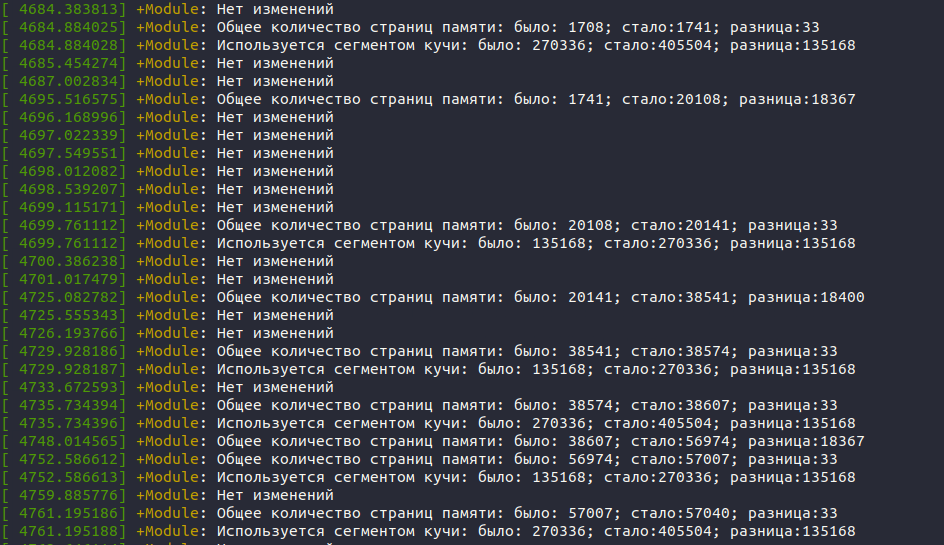
\includegraphics[width=1\textwidth]{img/analysis_program2.png}
		\caption{Демонстрация увеличение количества страниц при анализе описанной выше программы при увеличение кол-ва потоков}
		\label{fig:analysis_program2}}
\end{figure}

\section{Вывод}

В данном разделе был приведен анализ описанной выше программы.


\backmatter %% Здесь заканчивается нумерованная часть документа и начинаются ссылки и
%% заключение

\Conclusion % заключение к отчёту

В рамках выполнения работы решены следующие задачи.

\begin{enumerate}
	\item Рассмотрены основополагающие материалы, которые в дальнейшем потребовались при реализации загружаемого модуля ядра.
	\item Рассмотрены требования к программе.
	\item Был выбран язык программирования и среда разработки, а также представлены листинги.
	\item Был написан загружаемый модуль ядра.
	\item Была написана дополнительная анализируемая программа.
	\item Проведен анализ дополнительной анализируемой программы.
	\item Была написана вспомогательная программа.
	\item Проведен анализ количества выделяемых страниц в зависимости от количества выделяемой памяти.
\end{enumerate}


% % Список литературы при помощи BibTeX
% Юзать так:
%
% pdflatex report
% bibtex report
% pdflatex report

\bibliographystyle{gost780u}
\bibliography{report}





%\appendix   % Тут идут приложения

\end{document}